Before diving into the actual experiment built to test the hypothesis, this
chapter discusses and describes the method employed to model spiking
and artificial \gls{NN}s.

Both types of network are architecturally similar, and both are conceived from
the same physiological principles \autocite{dayan2001, russel2007, Nilsson2009, schmidhuber2014}.
The implementations, however, vary greatly.

To ensure internal and external validity in and between the two network types,
it is desirable that the models are as closely related from a theoretical and
practical perspective as possible.
Additionally, to test the hypothesis, it is required that both the artificial
and spiking models can be simulated on regular machine architecture, while
the spiking model requires a neuromorphic hardware platform.

An optimal approach would be to find a tool that leverages the similarities
of the network types, while integrating with the diverse simulated or emulated
targets.
That is, an abstract model of neural networks that can translate into
heterogeneous back-ends, while retaining a high degree of inter-model validity.

A number of general frameworks for artificial neural networks
exist\footnote{
  Among others, see \autocite{ONNX2018}, \autocite{PyTorch2018}, \autocite{TensorFlow2018},
  \autocite{Keras2018} and DyNet \autocite{Neubig2017}.
}, but none of them extend to the spiking domain.
Conversely a number of choices exist for neuromorphic modelling\footnote{
  %TODO: Find sources on internal IBM/Intel stuff
}, but they exclusively evaluate to neuromorphic or spiking neural network
backends \autocite{Jordan2018}.

Recently however, a domain-specific language (DSL) called Volr was developed
to construct reproducible \gls{NN} experiments
\autocite{Pedersen2018:volr}.
The DSL allows the modelling of sufficiently complicated models for
the purpose of this thesis, while providing a set of tools that permits the
model be sent and evaluated on both \gls{ANN} and \gls{SNN} targets.

Some work was required to fully support learning mechanisms on
neuromorphic hardware, and the DSL, as well as the tooling around it, has been
extended for the purpose of this thesis (see appendix \ref{appendix:volr})
The following section describes the architecture and principles of Volr in
detail.

\section{Volr}
Volr is a declarative language designed to model \gls{NN}.
Volr offers a trade-off between complete, but verbose, descriptions of small
networks and more general designs of large and complex networks, by separating
the network topologies from the detailed physiological properties of each
neuron or neuron population.

\subsection{Volr syntax}
This section defines the syntactical concepts of Volr step by step, beginning
with the general notion of an \textit{experiment}. For completeness the full
definition of the language can be found in appendix \ref{appendix:volr}.

\begin{figure}
  \label{fig:volr-ebnf}
  \begin{minipage}{0.9\linewidth}
    \begin{grammar}
      <experiment> = <stimuli> , <populations> , <responses> , <targets> ;
    \end{grammar}
  \end{minipage}
  \caption{EBNF of Volr}
\end{figure}

Figure \ref{fig:volr-ebnf} shows how an experiment is constructed. It consists
of four sub-components: A number of stimuli, neural populations, responses and
experiment targets.

\subsubsection{Experiment stimuli}
The stimuli describes the ``input'' of the model, either as data arrays directly
in the DSL or loaded via an external source.

\begin{figure}
  \label{fig:volr-ebnf-stimuli}
  \begin{minipage}{0.9\linewidth}
    \begin{grammar}
      <stimuli>  = <stimulus> , [ <stimuli> ] ;

      <stimulus> = 'stimulus' , [ <label> ] , <stimulus-source> ;

      <stimulus-source> = 'file: ' , <string>
        \alt 'array: ' , <number-list> ;
    \end{grammar}
  \end{minipage}
  \caption{EBNF of Volr}
\end{figure}


\subsubsection{Experiment populations}
The populations describe the architecture of the neural network itself,

\subsubsection{Experiment responses}
The responses are the recorded ``output'' of the model.

Both the populations
and the responses also describe their connectivity to either one or more
stimuli or population.

\subsubsection{Experiment targets}
Finally the targets describe one or more destination environments on which
to run the experiment. These are described in detail in section \ref{sec:volr-targets}.

\subsubsection{Block grammar}
The sub-components are constructed using the same declarative \textit{block}
structure shown in figure \ref{fig:volr-ebnf-block}.

\begin{figure}
  \label{fig:volr-ebnf-block}
  \begin{grammar}
    <block> ::= <block-type> ','
  \end{grammar}
\end{figure}


\subsection{Experimental validity}
... checks for valid/invalid experiments

\subsection{Volr semantics}
In practice a network is built by describing a graph.
The nodes in the graph consist of \texttt{populations} of neurons and the edges
are connection-set matrices to other populations \autocite{Djurfeldt2012}.
% TODO: Describe CSA
\texttt{Populations} can consist of any positive number of neurons and is
required to have at least one connection.
Connections can be recursive, resulting in a potentially cyclic graph.
Both the connections and the \texttt{populations} can be annotated with features
such as connection weight and neuron parameters (see \nameref{appendix:volr}).
The parameters are treated differently depending on the experiment target (see
sections \ref{sec:volr-NEST} and \ref{sec:volr-BrainScaleS}).

\section{Neural network simulation targets in Volr} \label{sec:volr-targets}

Volr exploits the structural similarities between \gls{ANN} and \gls{SNN} to
translate the model to both spiking and artificial network platforms (back-ends).

In the remainder of the chapter the three emulation back-ends, shown in figure
\ref{fig:volr}, are described:
a machine learning target for \gls{ANN}s and a neuron simulation target, as well
as a neuromorphic hardware target, for \gls{SNN}s.

\begin{figure}
  \centering
  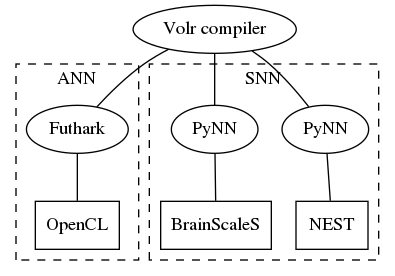
\includegraphics[width=0.6\textwidth]{images/volr-architecture.png}
  \caption{The translation from the Volr DSL to \gls{ANN} simulations in OpenCL via
    \gls{Futhark} and to \gls{SNN} simulations on \gls{NEST} and \gls{BrainScaleS}
    via the \gls{Myelin} middleware.
  }
  \label{fig:volr}
\end{figure}

\subsection{Translation to Futhark} \label{sec:volr-futhark}
Futhark is a functional data-parallel programming language \autocite{Henriksen2017}.
It offers a number of compilation targets such as \gls{OpenCL}, which is
particularly interesting for this thesis because of its capacity for hardware
acceleration.

The practical translation from the Volr model to Futhark is built on recurrent
\gls{ANN} with stochastic gradient descent backpropagation
\autocite{russel2007, schmidhuber2014}.
Each neuron population is considered as a single layer, whose connections are
determined by a connection matrix.

% Deal with recurrent connections
% Describe how this relates to layers

... To be continued ...

\subsection{Spiking neural network simulations via PyNN} \label{sec:volr-pynn}
The Python neural network simulation interface PyNN is designed as a
"simulator-independent language for building neuronal network models"
\autocite{PyNN2018}.
It aims to reduce the problem of diverse, and occasionally unique, descriptions
of neural network experiments for different simulation back-ends \autocite{Davison2009}.
PyNN has been adapted by a number of simulators, including the NEST simulation
platform and the neuromorphic BrainScaleS wafer system
\autocite{Davison2009, Helias2012, Schmitt2017}.

There are still simulator-dependent configurations that seems unlikely to be
adopted into PyNN in the immediate future\footnote{
  Particularly hardware mapping configurations are hard to abstract in a general
  interface.
}.
For that reason Volr provides simulation-specific PyNN scripts that can
interpret the model in the context of each simulation target.
A middleware, dubbed \gls{Myelin}, was invented to translate the \gls{NN} model
into a static intermediate representation in JSON.
The JSON standard was chosen for the task because of its concise syntax while
still retaining human readability.

The advantage of the static experiment representation being, that the experiment
easily a) transports to the target PyNN scripts without losing any information,
and b) duplexes between several experiment; the same experiment setup is
trivial to setup on multiple targets at once.

The correct execution of the experiments relies on the PyNN scripts to exploit
the simulator to represent the Volr model as accurately as possible.
Fortunately PyNN is designed to cover exactly such a use case, so properties
related to the \gls{NN} models itself (such as network topology and population
attributes) were faithfully reproduced across the simulators.
However, the simulators deviate in a number of ways that are relevant to
mention.
The following two sections explains the steps necessary to achieve accurate
experiment environments in \gls{NEST} and \gls{BrainScaleS}.

\subsubsection{Translation to PyNN} \label{sec:volr-translation}

\subsubsection{Translation to NEST} \label{sec:volr-NEST}
... To be continued ...
\subsubsection{Translation to BrainScaleS} \label{sec:volr-BrainScaleS}
... To be continued ...
